Encuentra el valor de la incógnita en el triángulo de la figura \ref{fig:angle_triangle_36}.

\begin{minipage}[t][5cm][b]{0.3\textwidth}
    \begin{figure}[H]
        \centering
        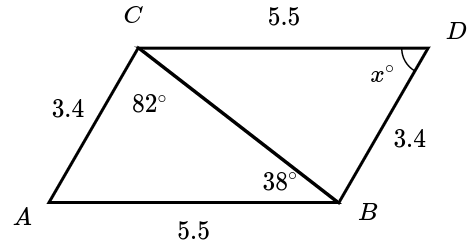
\includegraphics[width=0.9\linewidth]{../images/angle_triangle_36.png}
        \caption{}
        \label{fig:angle_triangle_36}
    \end{figure}
\end{minipage}\hfill
\begin{minipage}[t]{0.65\textwidth}
    \begin{solutionbox}{5cm}
        $\triangle ABC$ y $\triangle BCD$ tienen tres lados iguales. Comparten el lado
        $\overline{BC}$, las longitudes de $\overline{AB}$ y $\overline{CD}$ son iguales y las longitudes de
        $\overline{AC}$ y $\overline{BD}$ son iguales. Por lo tanto,
        $\triangle ABC$ y $\triangle BCD$  son congruentes.
        Los triángulos congruentes también tienen ángulos congruentes (iguales). Si superponemos estos dos triángulos, rotando
        $\triangle ABC$, observamos que el ángulo $x$ corresponde al
        $\angle BAC$ y $\angle BAC$ mide: \[x=180^\circ-82^\circ-38^\circ=60^\circ\]
    \end{solutionbox}
\end{minipage}
